\documentclass[a4paper,12pt]{article}

\usepackage[utf8]{inputenc}
\usepackage[T2A]{fontenc}
\usepackage[russian]{babel}
\usepackage{lmodern}
\usepackage{cmap}
\usepackage{amsmath,amsfonts,amssymb}
\usepackage{array}
\usepackage{colortbl}
\usepackage[svgnames,table]{xcolor}
\definecolor{taskred}{RGB}{170,0,0}
\definecolor{taskgreen}{RGB}{0,120,80}
\definecolor{taskblue}{RGB}{0,78,160}
\usepackage{graphicx}
\usepackage{tikz}
\usepackage{enumitem}
\usepackage{geometry}
\geometry{top=25mm,bottom=35mm,left=35mm,right=20mm}

\author{
Графические приёмы
Выполнил: Фамилия И.\,О. \\
Группа: группа
}
\title{Лабораторная работа по \LaTeX}
\date{\today}

\pagestyle{plain}
\setlength{\parindent}{0pt}
\setlength{\parskip}{0.35em}
\renewcommand{\arraystretch}{1.25}
\pagecolor{MintCream}

\newlength{\taskw}
\setlength{\taskw}{0.83\textwidth}
\newcommand{\taskbox}[2]{%
  \par\noindent\makebox[1.9em][r]{#1)}\hspace{0.6em}%
  \fcolorbox{black}{MistyRose}{%
    \begin{minipage}{\taskw}
      \vspace{0.55em}
      #2
      \vspace{0.55em}
    \end{minipage}%
  }%
  \par\vspace{0.9em}%
}

\begin{document}
\maketitle
\setcounter{section}{15}
\section{Задания}
\large

Написать в \LaTeX следующие фрагменты текста:

\taskbox{1}{%
Количество сочетаний можно вычислить по формуле
\[
C_n^m=\frac{\textcolor{taskblue}{n(n-1)\ldots(n-m+1)}}{\textcolor{taskgreen}{m!}}
\]
\textcolor{taskblue}{Синим цветом} выделено количество упорядоченных выборок из $n$ по $m$ элементов, а
\textcolor{taskgreen}{зеленым} --- количество возможных упорядочений.
}

\taskbox{2}{%
Формулу Эйлера можно получить, сравнивая степенные ряды для экспоненты, синуса и косинуса:
\[
 e^{ix}=\textcolor{taskred}{1}+\textcolor{taskgreen}{ix}+\textcolor{taskred}{-\frac{-x^2}{2!}}+\textcolor{taskgreen}{\frac{-i x^3}{3!}}+\textcolor{taskred}{\frac{x^4}{4!}}+\textcolor{taskgreen}{\frac{i x^5}{5!}}+\cdots
\]
\[
\cos x=\textcolor{taskred}{1+\left(\frac{-x^2}{2!}\right)+\left(\frac{x^4}{4!}\right)-\cdots}
\]
\[
 i\sin x=\textcolor{taskgreen}{i\left(x-\frac{x^3}{3!}+\frac{x^5}{5!}+\cdots\right)}
\]
}\taskbox{3}{%
Класс алгебр является многообразием тогда и только тогда, когда он замкнут относительно
\begin{itemize}[leftmargin=1.4em,itemsep=0.6em]
  \item \textcolor{taskred}{подалгебр},
  \item \textcolor{taskblue}{гомоморфизмов},
  \item \textcolor{taskgreen}{прямых произведений}.
\end{itemize}
В прямую сторону утверждение тривиально. В обратную сторону сначала доказывается аксиоматизируемость с использованием
\textcolor{taskgreen}{прямых произведений} и \textcolor{taskblue}{гомоморфизмов}. Затем --- аксиоматизируемость с помощью хорновских предложений с применением
\textcolor{taskgreen}{прямых произведений} и \textcolor{taskred}{подалгебр}. Наконец, --- аксиоматизируемость равенствами, применяя \textcolor{blue}{гомоморфизмы}.
}

\clearpage

\taskbox{4}{%
Начало таблицы Менделеева выглядит так:
\begin{center}
\setlength{\arrayrulewidth}{0.4pt}
\begin{tabular}{|>{\columncolor{Salmon!70}}c|*{6}{>{\columncolor{white}}c|}>{\columncolor{Violet!40}}c|}
\cline{1-1}\cline{8-8}
\cellcolor{Salmon!70}H & \multicolumn{6}{c|}{} & \cellcolor{Violet!40}He \\
\hline
\rowcolor{Salmon!70}Li & \cellcolor{SkyBlue!65}Be & \cellcolor{Gold!60}B & \cellcolor{Gold!60}C & \cellcolor{Gold!60}N & \cellcolor{Gold!60}O & \cellcolor{Orange!60}F & \cellcolor{Violet!40}Ne \\
\hline
\rowcolor{Salmon!70}Na & \cellcolor{SkyBlue!65}Mg & \cellcolor{Gold!60}Al & \cellcolor{Gold!60}Si & \cellcolor{Gold!60}P & \cellcolor{Gold!60}S & \cellcolor{Orange!60}Cl & \cellcolor{Violet!40}Ar \\
\hline
\end{tabular}
\end{center}
Цветами выделены: \textcolor{Salmon!80!black}{щелочные металлы}, \textcolor{SkyBlue!60!black}{щелочноземельные металлы},
\textcolor{Orange!70!black}{галогены}, \textcolor{Violet!60!black}{инертные газы}.
}

\taskbox{5}{%
При умножении матриц элемент \textcolor{taskgreen}{$c_{ij}$} произведения получается так: берется \textcolor{taskgreen}{$i$-ая строка} первой матрицы,
скалярно умножается на \textcolor{taskgreen}{$j$-ый столбец} второй:
\[
\left(\begin{array}{cc}
\cellcolor{taskgreen!18}1 & \cellcolor{taskgreen!18}3 \\
4 & 5
\end{array}\right)
\times
\left(\begin{array}{cc}
2 & \cellcolor{taskgreen!18}1 \\
3 & \cellcolor{taskgreen!18}{-2}
\end{array}\right)
=
\left(\begin{array}{cc}
11 & \cellcolor{taskgreen!18}{-5} \\
23 & -6
\end{array}\right)
\]
}

\taskbox{6}{%
Таблица производных/первообразных для простейших функций:
\begin{center}
\setlength{\tabcolsep}{12pt}
\rowcolors{2}{white}{gray!10}
\begin{tabular}{>{\centering\arraybackslash}p{0.23\textwidth}>{\centering\arraybackslash}p{0.22\textwidth}>{\centering\arraybackslash}p{0.28\textwidth}}
\hline\hline
Функция & Производная & Первообразная \\
\hline
const & $0$ & $x+\mathrm{const}$ \\
$x^k\,(k\neq -1)$ & $k x^{k-1}$ & $\dfrac{x^{k+1}}{k+1}+\mathrm{const}$ \\
$\dfrac1x$ & $-\dfrac1{x^2}$ & $\ln|x|+\mathrm{const}$ \\
$e^x$ & $e^x$ & $e^x+\mathrm{const}$ \\
$\sin x$ & $\cos x$ & $-\cos x+\mathrm{const}$ \\
$\cos x$ & $-\sin x$ & $\sin x+\mathrm{const}$ \\
\hline
\end{tabular}
\end{center}
}

\clearpage

\taskbox{7}{%
При линейных преобразованиях круг:
\begin{center}
\begin{tikzpicture}[scale=1]
  \fill[blue] (0,0) circle[radius=1.55cm];
\end{tikzpicture}
\end{center}
превращается в эллипс:
\begin{center}
\begin{tikzpicture}[scale=1]
  \fill[blue] (0,0) ellipse[x radius=3.2cm,y radius=1.55cm];
\end{tikzpicture}
\end{center}
}

\clearpage

\taskbox{8}{%
Псевдосфера --- поверхность постоянной отрицательной кривизны выглядит следующим образом:
\begin{center}
\begingroup\setlength{\fboxsep}{0pt}\colorbox{white}{
\includegraphics[width=0.82\linewidth]{images/pseudosphere.png}}\endgroup
\end{center}
Она получается вращением трактрисы:
\begin{center}
\begingroup\setlength{\fboxsep}{0pt}\colorbox{white}{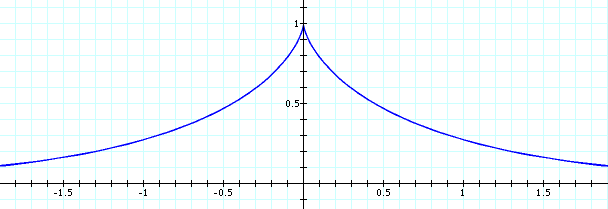
\includegraphics[width=0.82\linewidth]{images/tractrix.png}}\endgroup
\end{center}
вокруг асимптоты.
}

\clearpage

\taskbox{9}{%
Если график гиперболы, записанный с помощью классического уравнения $x^2-y^2=1$:
\begin{center}
\begingroup\setlength{\fboxsep}{0pt}\colorbox{white}{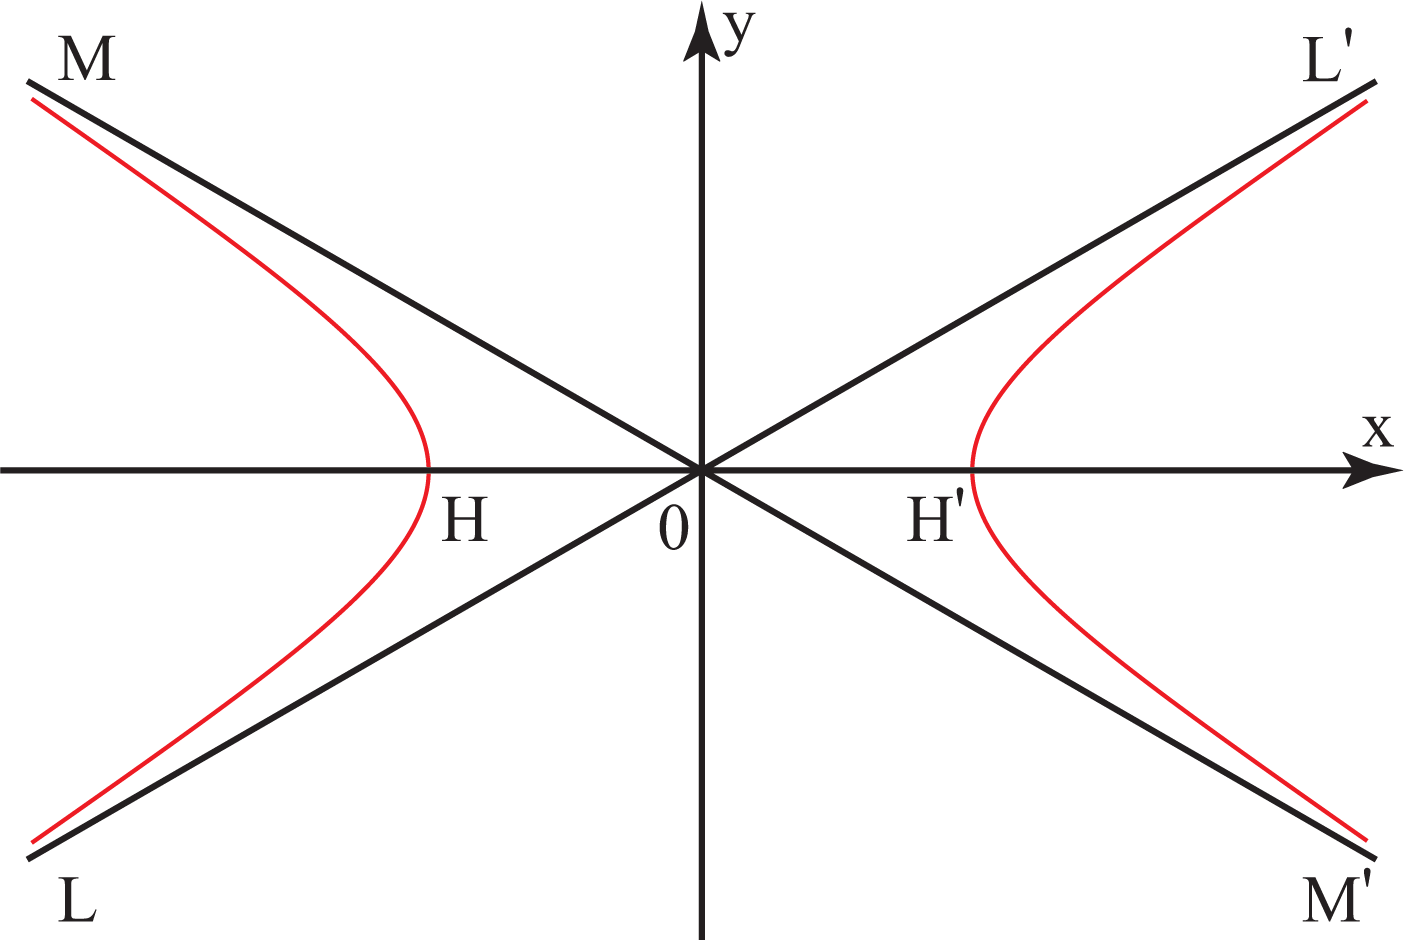
\includegraphics[width=0.82\linewidth]{images/hyperbole1.png}}\endgroup
\end{center}
повернуть на $45^\circ$, получится график гиперболы в асимптотах $xy=1$:
\begin{center}
\begingroup\setlength{\fboxsep}{0pt}\colorbox{white}{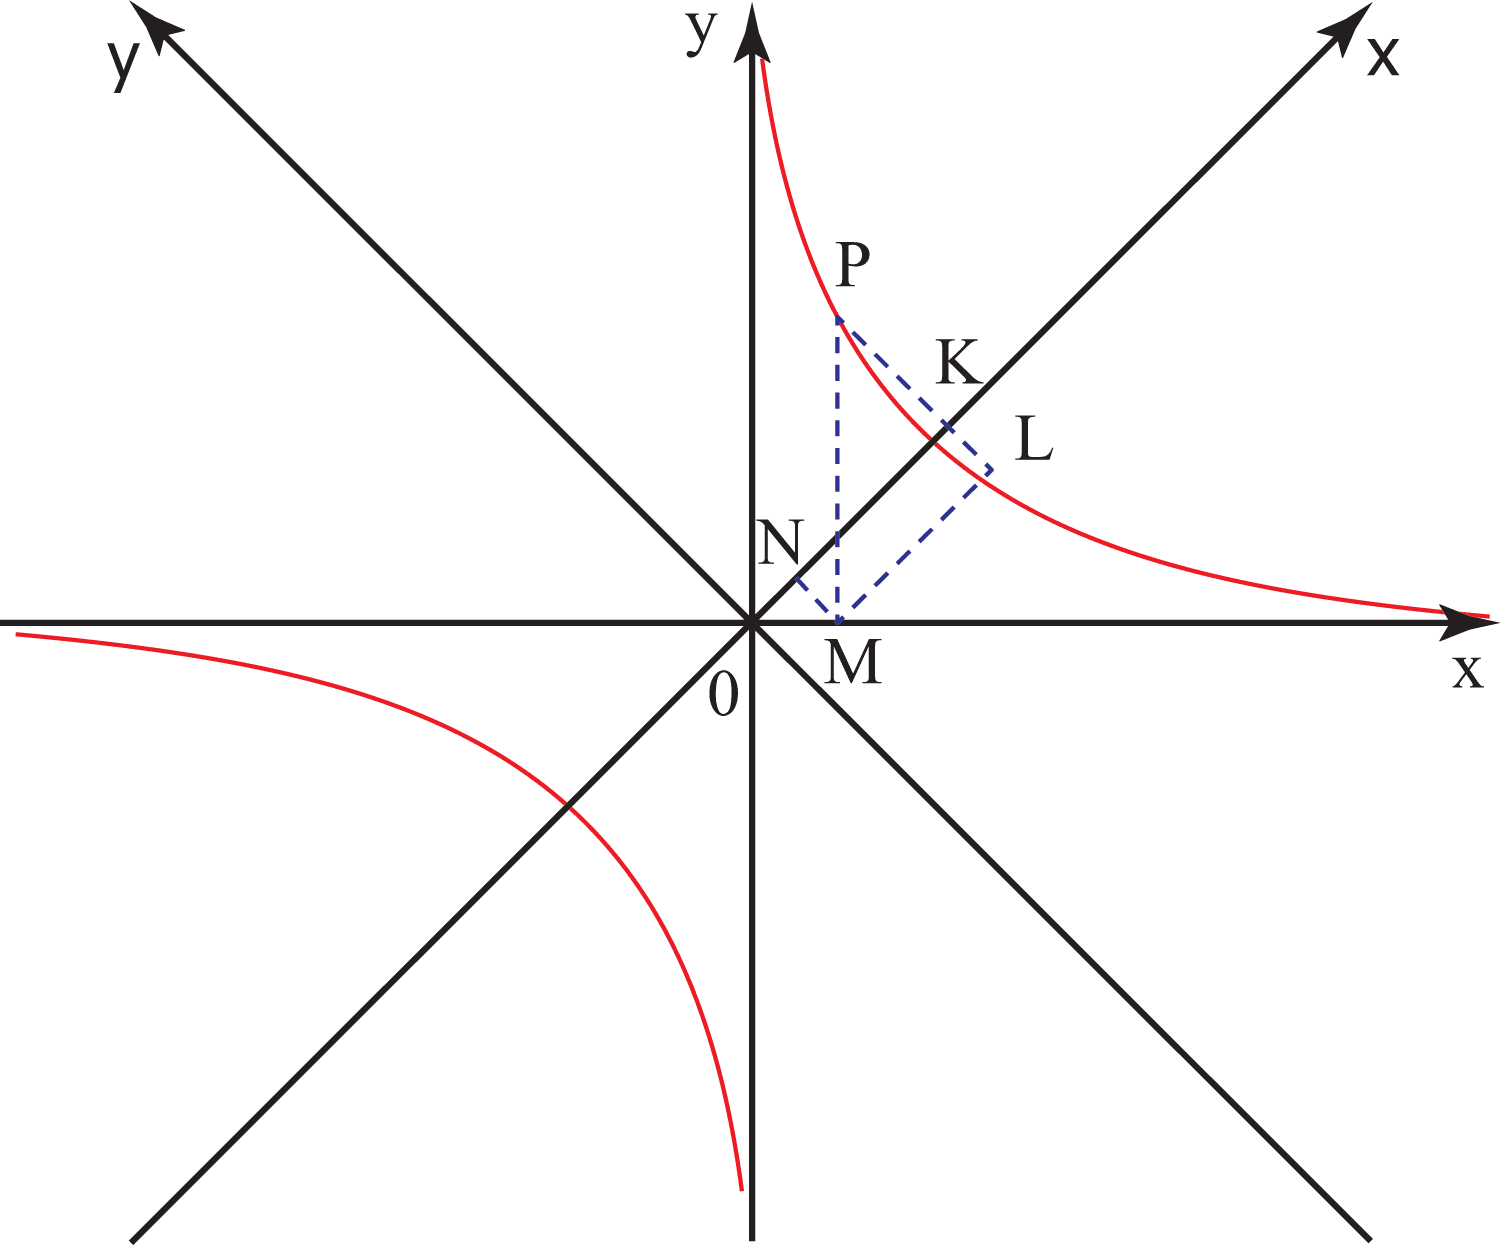
\includegraphics[width=0.82\linewidth]{images/hyperbole2.png}}\endgroup
\end{center}
}

\taskbox{10}{%
Циклоиду:
\begin{center}
\begingroup\setlength{\fboxsep}{0pt}\colorbox{white}{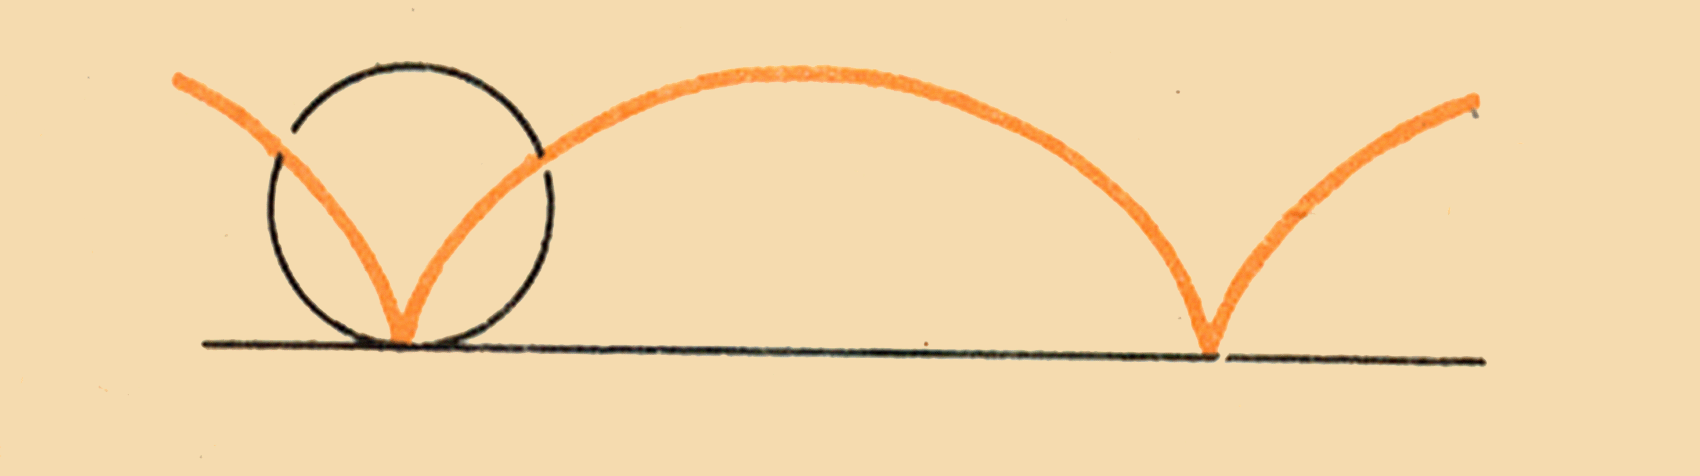
\includegraphics[width=0.82\linewidth]{images/cycloid.png}}\endgroup
\end{center}
можно получить как график движения точки окружности при ее качении по прямой (файл).
}

\taskbox{11}{%
Используя фокальные свойства эллипса $F_1X^2+F_2X^2=\mathrm{const}$:
\begin{center}
\begingroup\setlength{\fboxsep}{0pt}\colorbox{white}{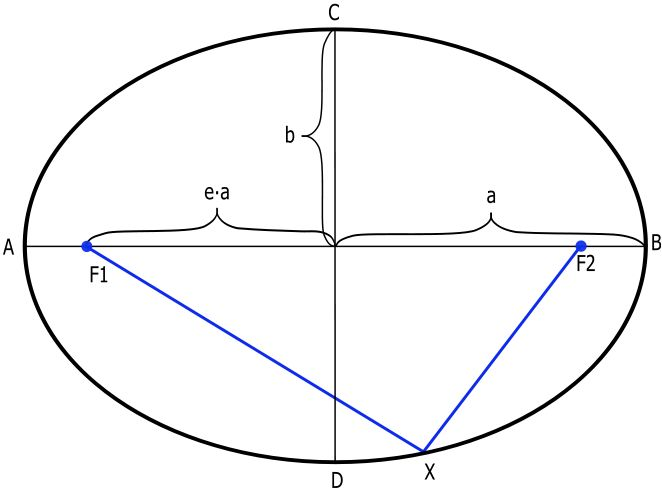
\includegraphics[width=0.82\linewidth]{images/ellipse2.png}}\endgroup
\end{center}
его легко построить:
\begin{center}
\begingroup\setlength{\fboxsep}{0pt}\colorbox{white}{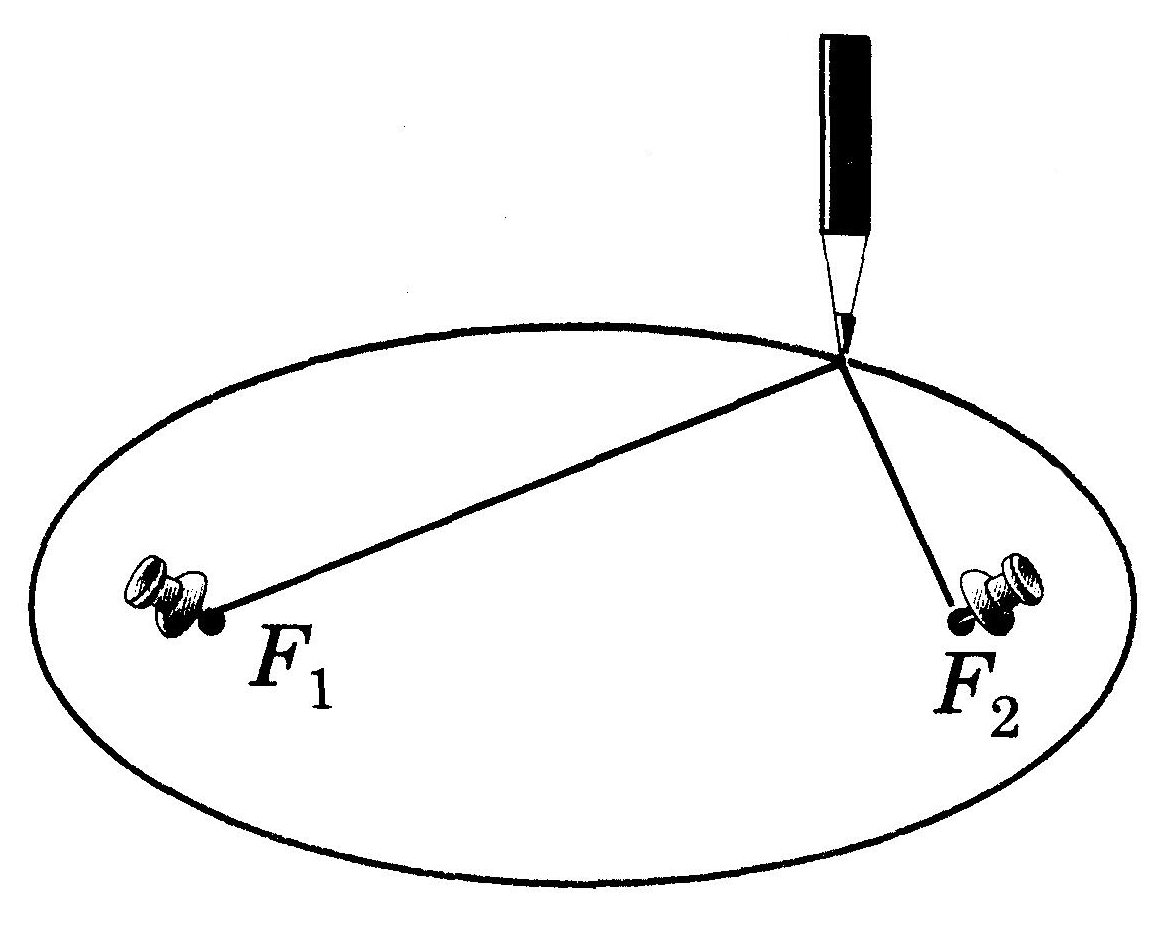
\includegraphics[width=0.82\linewidth]{images/ellipse1.png}}\endgroup
\end{center}
}

\taskbox{12}{%
Рассмотрим произвольную гладкую кривую:
\begin{center}
\begin{tikzpicture}[scale=1.0]
  \draw[line width=1.5pt] plot[smooth] coordinates {(0,0) (0.6,1.7) (1.2,2.9) (1.9,3.1) (2.7,2.4) (3.4,1.5) (4.1,1.0) (4.9,1.2) (5.7,1.8) (6.5,2.5) (7.2,2.9)};
\end{tikzpicture}
\end{center}
}
\end{document}